%!TEX root = ../../main.tex

\chapter{Modellhafte Darstellung zur Evaluierung}

\section{Versuchsaufbau}

\subsection{Motorenmodell}

\subsection{Hardwaremodell}

\section{Technische Umsetzung}

\subsection{Detektion des Propellerblattes}
Detektion des Propellers notwendig, da sonst nur eine Unwuchtdetektion möglich ist, aber keine Unwuchtlokalisierung
Im Endeffekt muss der Arduino in der Lage sein exakt sagen zu können, wann einer der beiden Seiten des Propellers an ihm vorbei kam
Es ist nicht notwendig beide Seiten des Propellers individuell erkennen zu können, da auf die Andere Seite Rückschlüsse gezogen werden können
Beide Seiten individuell erkennen zu können bringt allerdings vorteile im bereich der Zuordnung der Messergebnisse der Unwucht

\subsubsection*{Theoretische Vorgehensweise}
Markierung einer Seite des Propellers durch Anmalen oder durch Beklebung
Verschiedene Sensoren testen, welche diese angebrachten Beklebungen, bzw. die angemalten Flächen erkennen können

\subsubsection*{Vergleich zwischen Sensoren}
Detektion des Propellers könnte auf zwei Arten erfolgen:
- Detektion mittels eines Lichtsensors:
-- Eine Seite des Propellers wird hierbei schwarz angemalt / schwarz beklebt (auf jedenfall verdunkelt) um das Messergebnis zu verdeutlichen
-- Misst der Lichtsensor nun eine "deutliche" Verdunkelung (relativ zu den anderen Lichtwerten) kam der markierte Propeller vorbei und kann somit lokalisieren werden
-- Verwendeter Lichtsensor: Adafruit TSL2591
--- Dieser Lichtsensor bot ein paar coole Features weshalb man sich für diesen entschieden hat:
---- Sehr hohe Lux Reichtweite, weshalb Einsatz fast überall möglich
---- Differenziert beim Messen / Auslesen zwischen IR Licht- und komplettem Lichtspektrum, somit können Lichteinflüsse (durch helle Sonneinstrahlung) vermieden werden
---- Bietet Interrupt Schnittstelle wodurch deutliche Komplexitätsreduzierung
- Detektion mittels einer IR-Reflektions-Schranke:
-- Eine Seite des Propellers wird wiederum schwarz angemalt / schwarz beklebt, bzw. wenn der Rotor bereits zu dunkel ist, wird eine Seite mit reflektierender Farbe angemalt / beklebt
-- Misst der IR-Reflektions-Sensor nun eine Reflektion (direkt durch Propeller oder durch reflektierender Auftrag auf Propeller) ist eine Seite des Propellers lokalisiert worden
-- Verwendeter IR-Reflektions-Sensor: https://www.adafruit.com/product/2349
--- Features:
---- Deutlich einfacherer Aufbau im Gegensatz zum Lichtsensor
---- Abtastraten / Messergebnisse in einer deutlich höheren Geschwindigkeit als beim Lichtsensor

\subsubsection*{Probleme bei der Detektion}
Weshalb der Lichtsensor nicht funktioniert hat:
- Der Lichtsensor verwendet einen kleinen Mikrocontroller, welcher die Werte der beiden Lichtdioden über einen Zeitraum von mindestens 100ms aggregiert
- Er ist damit zu langsam (Vergleich: Eine Umdrehung des Propellers benötigt ca. 24ms)
- Dieses Verhalten wurde erst nach dem Kauf des Lichtsensors entdeckt
Probleme / Macken des IR-Reflektions-Sensors:
- Ständige Probleme mit Abstand, da Sensor nur zwischen 2-10mm funktioniert
- Ständige Probleme durch Sonneneinstrahlung und ein damit in verbindung stehendes fehlverhalten der detektion des Propellers (Propeller kam oftmals vorbei und wurde nicht erkannt)
- Detektion des Propellers ist mit diesem Sensor allerdings möglich !!

\subsection{Detektion der Unwucht}

\subsubsection*{Theoretische Vorgehensweise}
Besitzt ein Propellerblatt eine Unwucht, erzeugt dieser deutlich spührbare Vibrationen am Motorblock.
Diese Vibrationen sollen mithilfe eines 3-Achsen Sensors gemessen werden.
Je nach Auslenkung des Motorblockes kann hierdurch eine Unwucht detektiert werden.
Desweiteren kann unter Berücksichtigung der Propellerdetektion, eine Unwuchtlokalisierung erfolgen. 

Um solch eine Unwucht zu erzeugen, werden wie in Abbildung \ref{fig:propeller-mit-unwucht} gezeigt, mehrere Propeller mit unterschiedlichen Gewichten, bzw. identischen Gewichten jedoch an unterschiedlichen Stellen präpariert.
\begin{figure}[H]
	\centering
	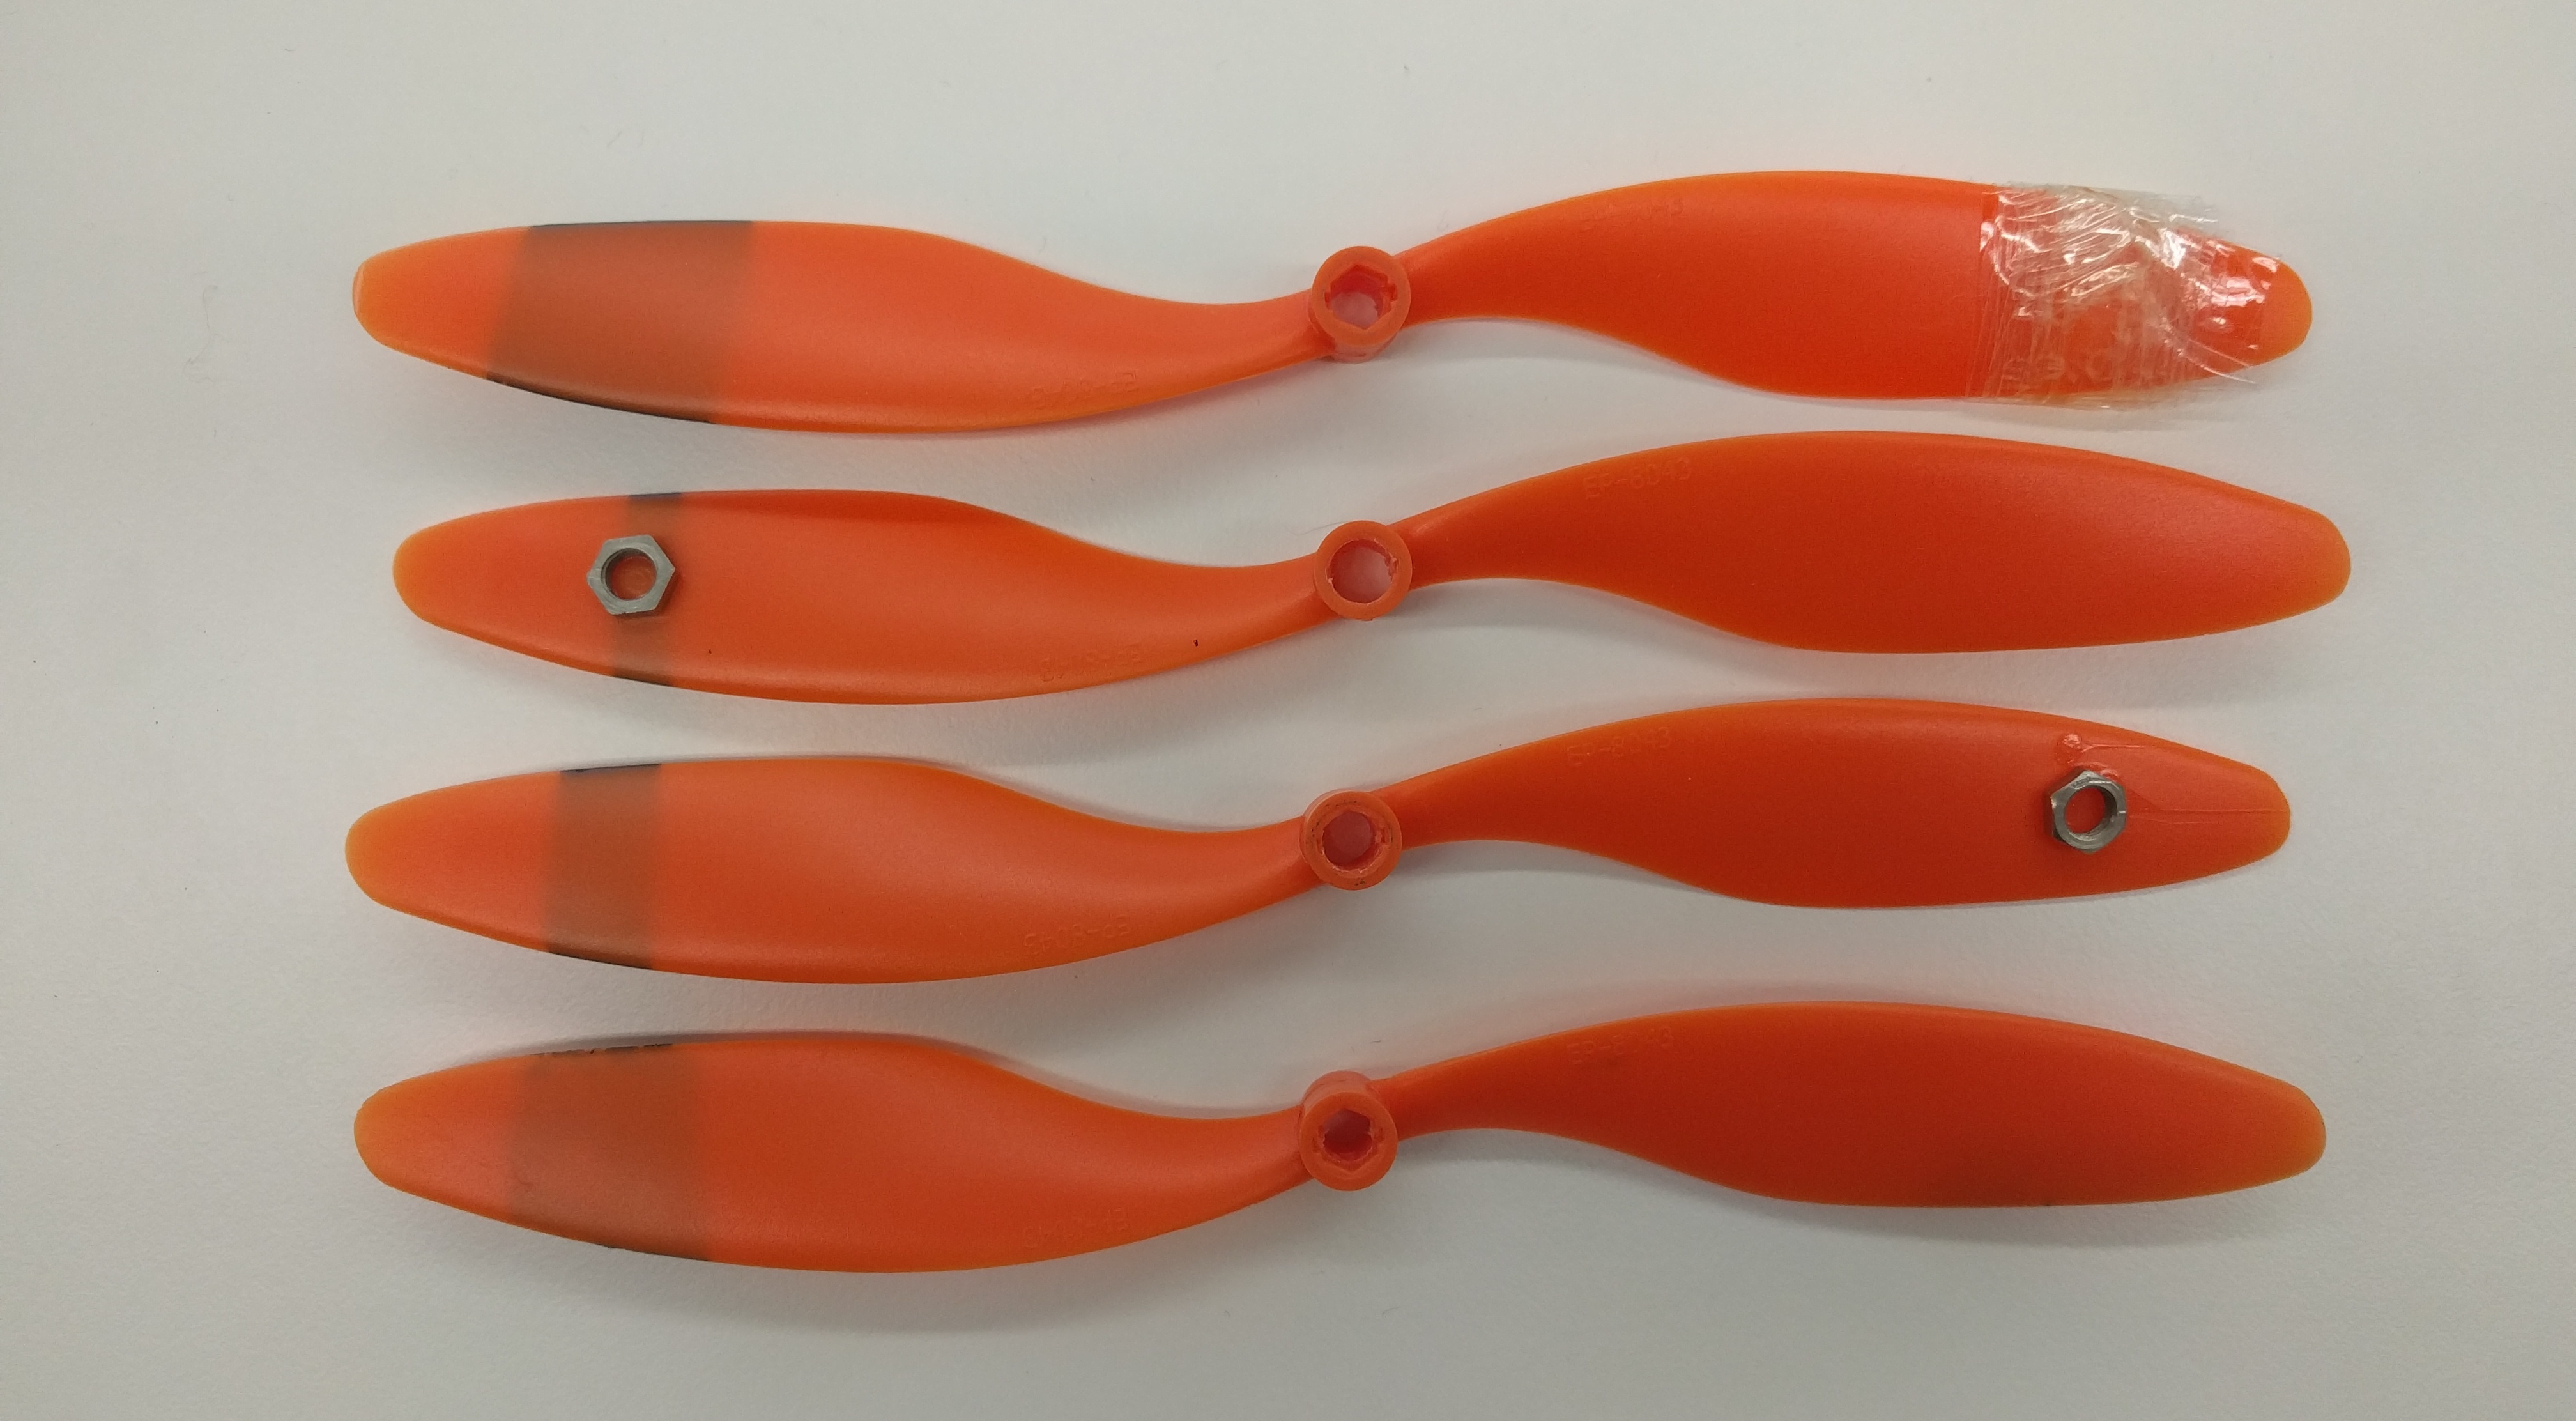
\includegraphics[width=0.9\textwidth]{images/chapter/03/propeller-mit-unwucht.png}
	\caption{Propeller mit unterschiedlichen Unwuchten}
	\label{fig:propeller-mit-unwucht}
\end{figure}

\subsubsection*{Sensortechnologie}
Als 3-Achsen Sensor soll der LSM9DS1 9-DOF Sensor von Adafruit eingesetzt werden.
\begin{figure}[H]
	\centering
	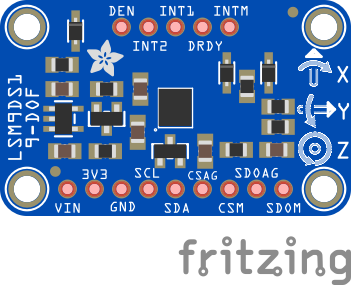
\includegraphics[width=5cm]{images/chapter/03/9-dof.png}
	\caption{Schematische Darstellung des verwendeten Sensors}
\end{figure}
Dieser ist mit 4 verschiedenen Sensoren ausgestattet:
\begin{itemize}
	\item Beschleunigungssensor (Beschleunigung des Sensors in drei Richtungen)
	\item Gyroskop (Ausrichtung des Sensors)
	\item Magnetometer (Lage in Abhängigkeit des Erdmagnetfeldes)
	\item Temperatursensor
\end{itemize}

\subsubsection*{Messung der Unwucht}
Hier kommen dann Bilder rein und wir erklären und diskutieren die Ergebnisse dann, oder?

\subsubsection*{Probleme bei der Detektion}
Nachfolgende Probleme traten bei der Verwendung des Sensors auf:
- Das Auslesen der Sensordaten dauert zu lange. Es ist möglich 2-3 Messergebnisse (Variation hängt von Gewicht des Propellers ab) innerhalb einer Umdrehung (~20ms) des Propellers zu erhalten. Ein Versuch dieses Verhalten zu verbessern bestand darin die Verbindungsgeschwindigkeit zwischen \textit{Arduino} und Sensor zu erhöhen. Die Verbindung zwischen den beiden Geräten findet über die Schnittstelle I\textsuperscript{2}C im normalen Modus statt. Durch Manipulation der \textit{twi.h}, eine Header-Datei der Arduino-Bibliothek \textit{Wire.h}, welcher die Verbindungsparameter für die I\textsuperscript{2}C-Schnittstelle steuert, war es möglich die Verbindung im Fast-Mode zu betreiben. Damit wurde die Anzahl an Messergebnisse pro Umdrehung von 2-3 auf 3-5 Messungen erhöht. Dies ist aber weiterhin zu wenig um eine konkrete Entscheidung über die Lokalisation der Unwucht treffen zu können.
Es existiert eine weitere Möglichkeit den Sensor auf eine höhere Messrate zu bekommen, welche im Datenblatt jedoch nur sehr kurz und knapp erklärt ist. Hierbei ist es möglich das Gyroskop des Sensor abzuschalten und den Beschleunigungssensor mittels eines "Burst-Modus" (multiple reads) auszulesen. Den Sensor in diesen Modus zu setzen und auszulesen war allerdings aufgrund Mangel des technischen Verständnisses und der Datenblatterklärung nicht möglich.
Es kann davon ausgegangen werden, dass die benötigte Zeit für die Messung der Sensoren bei dem eingesetzten Sensor schon intern zu lange dauert. Die Empfehlung (für zukünftige Projekte ?) liegt daher auf dem Einsatz von anderen Sensoren, welche für diesen Einsatzzweck besser geeignet sind. Ein Beispiel hierfür ist der Bosch BMA180. Dies ist ein dreiachsichger Beschleunigungssensor, welcher intern mit einer Messgeschwindigkeit von 1200Hz operieren kann. Damit kommt dieser Sensor auf ein komplett neues Messergebniss alle 417$\mu$s (Quelle: http://irtfweb.ifa.hawaii.edu/~tcs3/jumpman/jumppc/1107-BMA180/BMA180-DataSheet-v2.5.pdf). Hiermit sind bei einer Umdrehungszeit von ~20ms bis zu 48 Messergebnisse möglich, welche wahrscheinlich ausreichend sind für eine Aussage über die Unwuchtlokalisierung. Eine weitere Möglichkeit für den Ersatz des Sensor wäre der Einsatz einer inertialen Messeinheit (englisch \textit{inertial measurement unit}, IMU). Dies ist meist eine räumliche Kombination von mehreren Sensoren, welche auch Einsatz in heutigen Drohnen finden. Ob sich diese für den hier benötigten Einsatz verwenden liesen ist nicht bekannt und müsste weiter recherchiert werden.
